
\section{HIJSON Toolkit}\label{hijson-toolkit}

The HIJSON Toolkit is a software module that implements common
operations and transformations on HIJSON documents. Written in
\emph{JavaScript} language, it has been built to be deployed in the web
environment. It is \emph{modular} and entirely \emph{isomorphic},
i.e.~can run on the server as well as on every client. Working in the
web environment, the Toolkit benefits of the fertility as regards the
software development in this field: it takes advantage of libraries and
frameworks such as \emph{Ract}, ``the JavaScript library for building
user interfaces'' by Facebook, and \emph{Three.js} a framework to deal
with \emph{WebGL} tecnologies.

The Toolkit realizes the instantiation and extension logic of a HIJSON
document, and realize a multistage transformation pipeline that, as required,
can be used entirely or only in part.

\subsection{Processing pipeline}\label{hijson-processing-pipeline}

The HIJSON processing pipeline relizes the sequence of preliminary
transformations that have to be applied to a HIJSON document before any
futher operation. It is not strictly required to complete each stage of
the pipeline: the exit stage dipends on the specific use case.

The application of the transformation pipeline has a double aim. The first one
consists in generating the graph of valid paths between all the interesting
HIJSON elements. The second objective is the generation of one \emph{GeoJSON}
document for each storey of the building described by the HIJSON document. In
this way a bidimensional plant for each level of the building can be provided
and visualized through any compliant GeoJSON viewer.

HIJSON processing pipeline (as pictured in figure AGGIUNGERE
RIFERIMENTO) is composed by 6 elaboration stages. In the following are
detailed operations excecuted by each stage, which are, in the order:
\emph{validation}, \emph{georeferencing}, \emph{parsing}, \emph{graph
paths generation}, \emph{2D layers generation}, \emph{marshalling}.

\begin{figure}[!htbp]
\centering
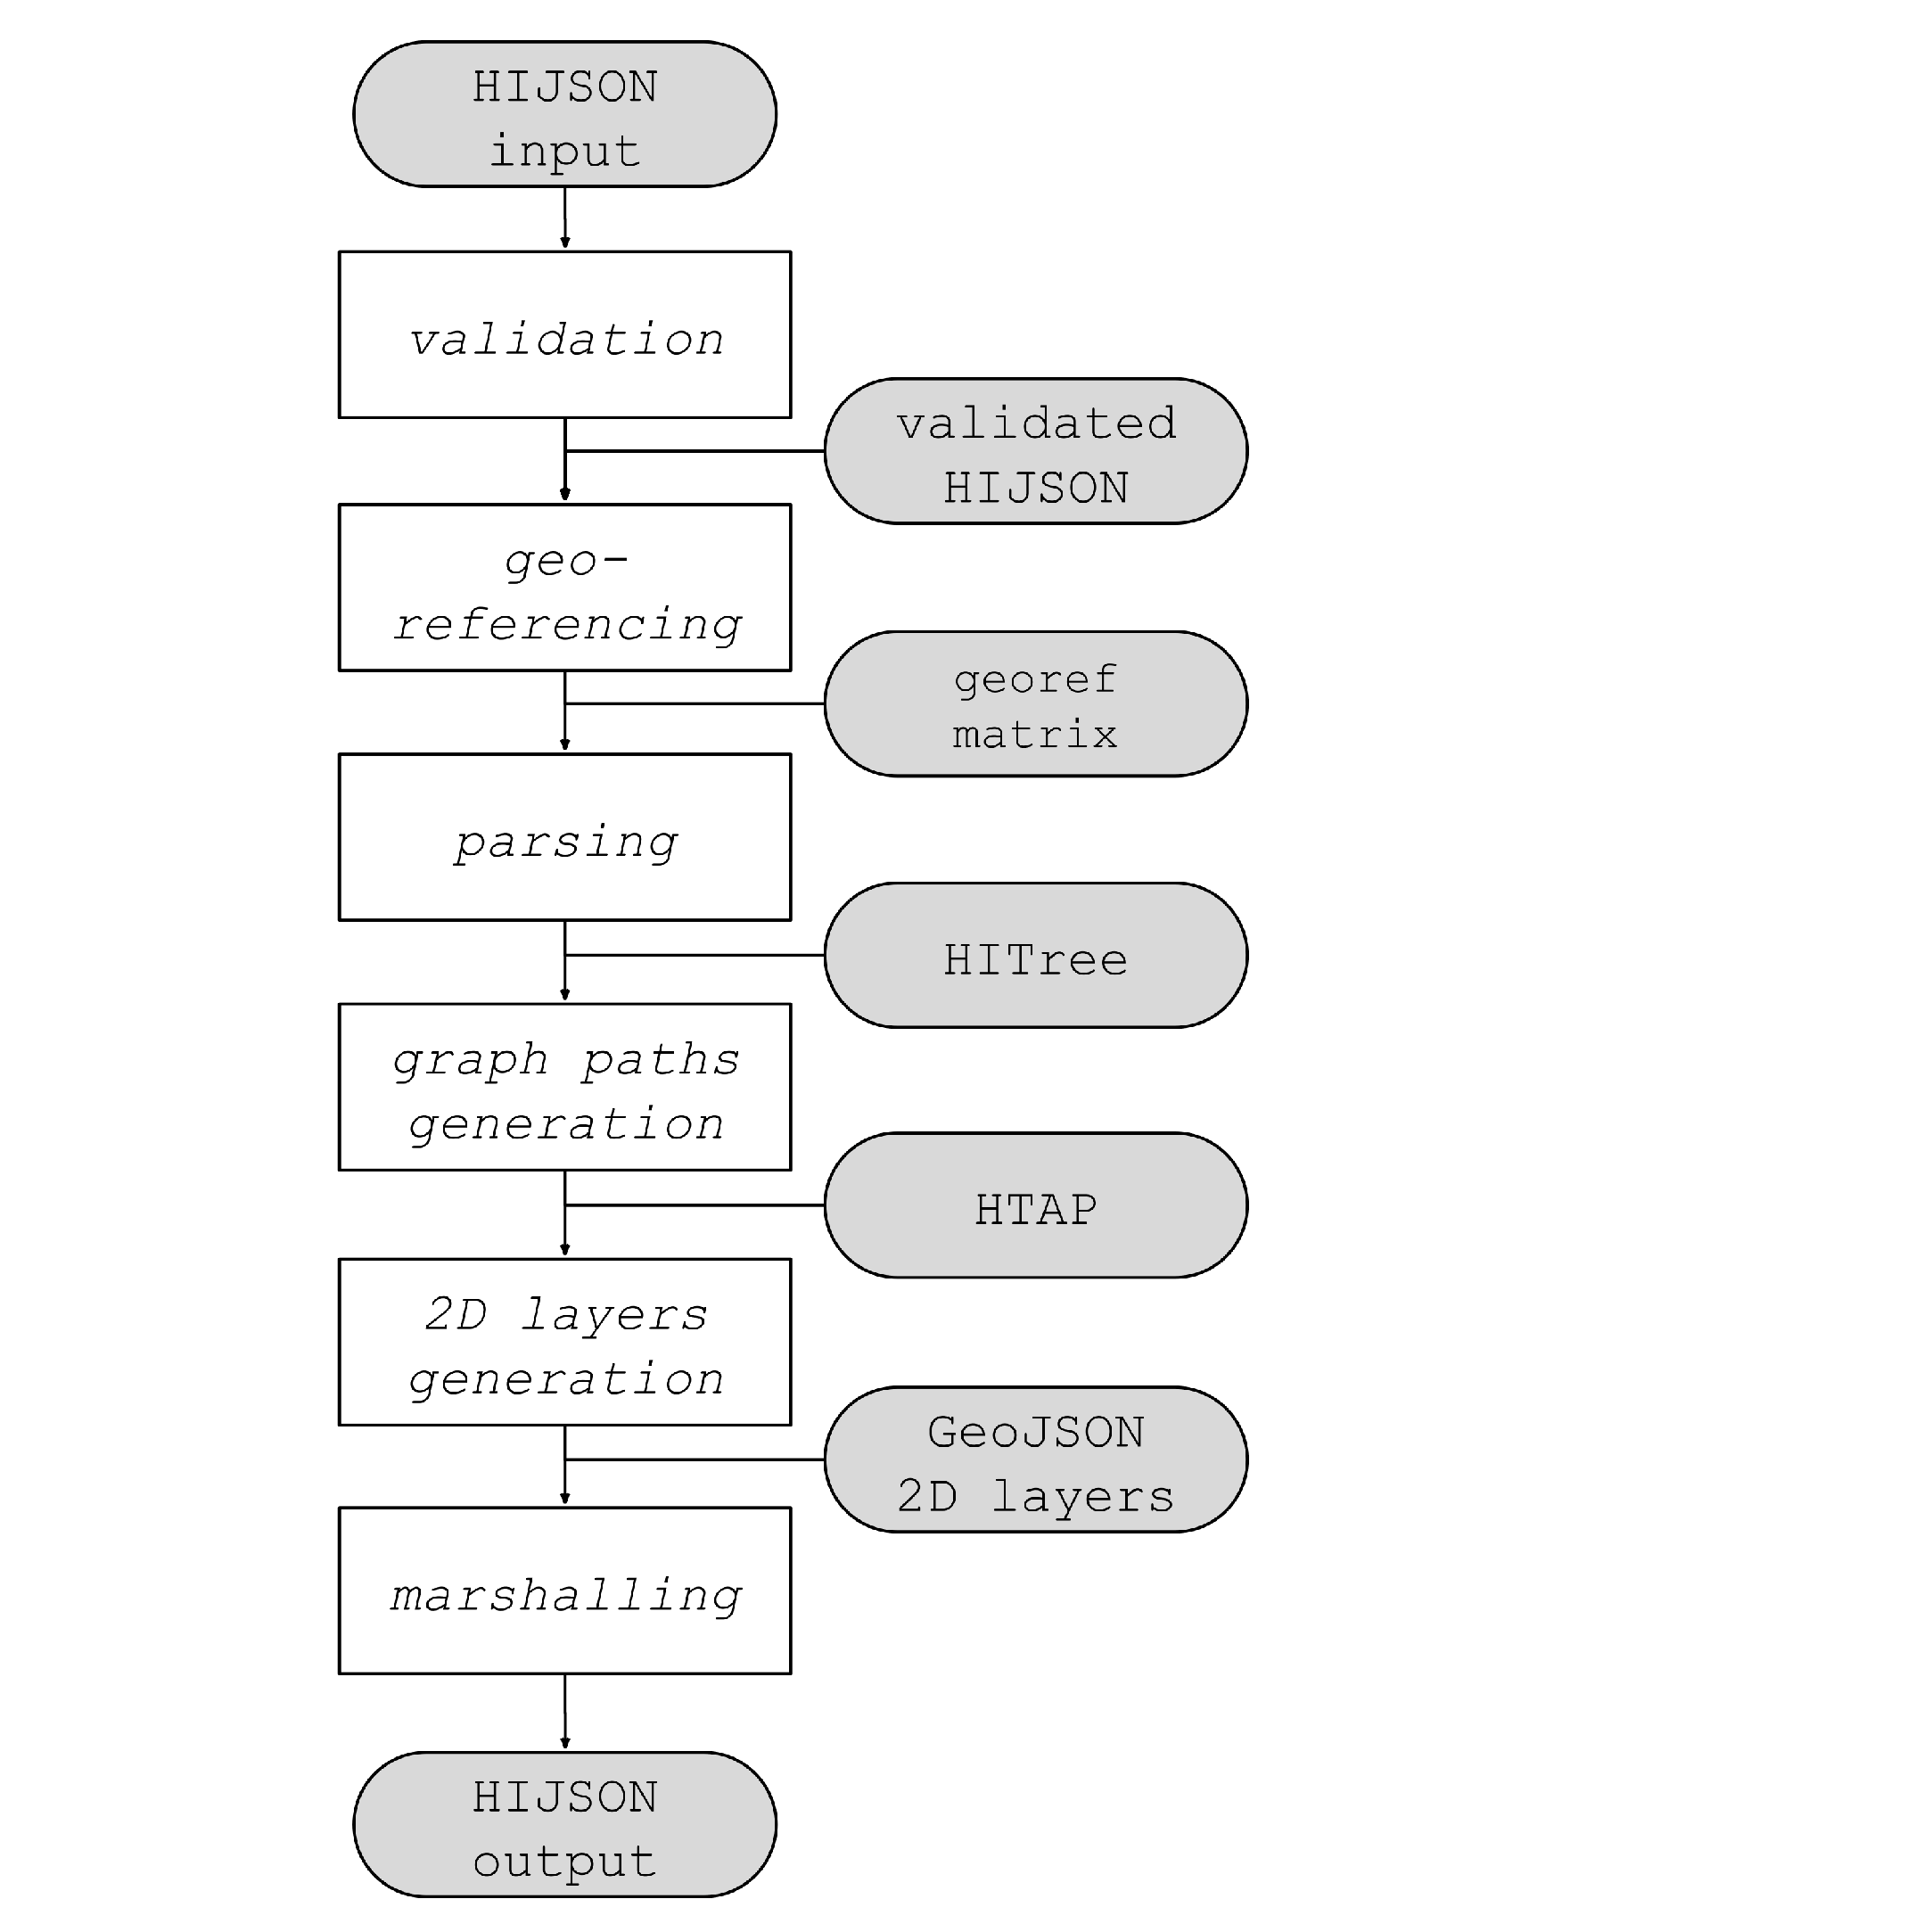
\epsfig{file=images/pipeline.eps, height=0.4\textwidth}
\caption{HIJSON processing pipeline}
\label{fig:pipeline}
\end{figure}

\begin{enumerate}
\def\labelenumi{\arabic{enumi}.}
\itemsep1pt\parskip0pt\parsep0pt
\item
 \textit{\texttt{validation}} - The first one is the validation stage. In
  order to begin with the effective transformations the input HIJSON  document
  must be compliant with the format syntax and structure requirements.   In the
  case the validation stage fails, processing aborts and do not continue to
  following stages. If  the stage success, the output for the next stage is a
  validated  HIJSON.

\item
 \textit{\texttt{georeferencing}} - In the second stage, in order to allow
 for continuous outdoor/indoor navigation, the system needs to compute
 the georeferencing matrix, a linear operator able to transform local
 coordinates into global coordinates (referred to world coordinate
 system as latitude and longitude misures) and viceversa. This task is
 accomplished by solving a linear system obtained from information
 contained in HIJSON configuration part and precisely from the
 correnspondance of three real word points to three points included
 into the HIJSON document.
\item
 \textit{\texttt{parsing}} - The parsing stage, takes the validated and
 georeferenced HIJSON as its input, that as illustrated before can be
 thought of as a list of HIJSON Elments, parses them and produce an
 istance of HIJSON Tree. The HIJSON Tree is an object in memory
 representing the tree hierarchical structure of the building described
 by the HIJSON document.
\item
 \textit{\texttt{graph paths generation}} - The fourth stage is in charge
 of the generation of the graph paths. The algorithm to achieve such a 
 goal is introduced below. The graph paths will be
 useful afterwards to compute valid paths from couple of point of
 interest on the graph. Once the graph paths has been computed, the
 input HIJSON Tree is augmented with paths information, becoming what
 has been called an HTAP (HIJSON Tree Augmented with Paths).
 Augmentation always takes place as leaf nodes added as children of a
 specific level (e.g. ``room'').
\item
 \textit{\texttt{2D layers generation}} - The fifth stage is the
 generation of GeoJSON layers. For each storey of the building, the Toolkit generates one
 geoJSON layer that will be use for the creation of a 2D map. Each layer
 contains only the children of a `level' node of the HIJSON Tree. 
 The presence of a specific element inside the layer can be finely tuned 
 by means of a boolean value. Every element has geographical coordinates
 calculated by the transformation matrix with regard to the local
 coordinates of the HIJSON Element.
\item
 \textit{\texttt{marshalling}} - The last stage is responsible of execute
 a serialization of the the transformed data. Tasks like breaking
 dependency-loops and stringification are performed. This stage is
 useful mainly serverside, as and the output is stored ready to be
 served to any requiring client.
\end{enumerate}

\subsubsection{Algorithmics: automatic generation of valid paths}\label{algorithmics-automatic-generation-of-valid-paths}

The fourth stage of the processing pipeline is responsible for the
generation of a graph of valid paths through the entire model
represented by the intput HIJSON document. The graph generated according
to the algorithm described in the following, although not optimal,
ensures a complete coverage of the surface while limiting the numebr of
generated nodes. Resulting graph is weigthed on the edges with nodes
distances and each node represents alternatively:

\begin{enumerate}
\def\labelenumi{\alph{enumi}.}
\itemsep1pt\parskip0pt\parsep0pt
\item
 standard path node, i.e.~a junction node or possibly an endpoint of a
 path;
\item
 connection node, used as subproblem composing element in the divide et
 impera approch adopted (as described below).
\item
 element nodes ie. HIJSON Element (whose HIJSON Class explicitly grants
 his presence in the graph), typically an endpoint of a path;
\end{enumerate}

Such a graph allows for calculations of directions between any two given
nodes. Although different approaches have been explored \cite{6999103}, 
a very classical solution has been selected in this case, so directions 
are actually computed clientside applying the Dijkstra's shortes route 
algorithm on the graph. 

Taking advantage of the hierarchical structure of the HIJSON document,
and according to the divide et impera approach, the problem of the graph
paths generation is splitted in several sub-problems which consist in
the computation of the sub-graphs relative to each room, or more
generally ambience. The sub-graphs are then linked together through the
connection nodes (which in most cases represents doors). The resolution
of each sub-problem (as depicted in figure \ref{fig:graph-generation}), 
is composed by 4 phases:

\begin{enumerate}
\def\labelenumi{\arabic{enumi}.}
\itemsep1pt\parskip0pt\parsep0pt
\item
 Computation of the walkable area of the ambience: this task is
 accomplished subtracting area of the possibly encumbrances to the area
 of the ambience; the result is tipically a surface with holes;
\item
 Triangulation of the walkable area: the computed surface is
 triangulated taking into account the presence of holes;
\item
 Identification of graph nodes: for each triangle side completely
 internal to the area, its midpoint is selected as standard path node;
\item
 Junction of nodes: nodes relative to the same triangle are then linked
 together; both element nodes and connection nodes (i.e.~doors) are
 linked to the nearest node in the ambience (i.e.~room).
\end{enumerate}

\begin{figure*}[!htbp]
 \centering
 \begin{subfigure}[b]{0.235\textwidth}
 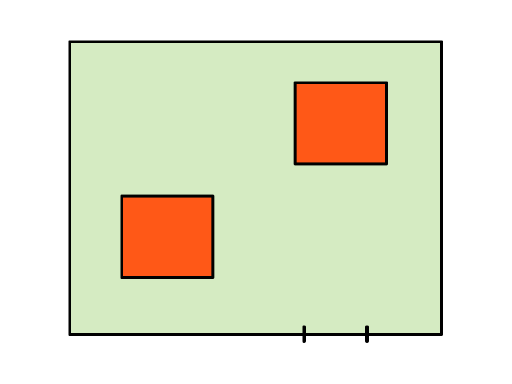
\includegraphics[width=\textwidth]{images/graph-generation/single/graph-generation-1}
 \caption{}
 \label{fig:graph-generation-a}
 \end{subfigure}
 ~
 \begin{subfigure}[b]{0.235\textwidth}
 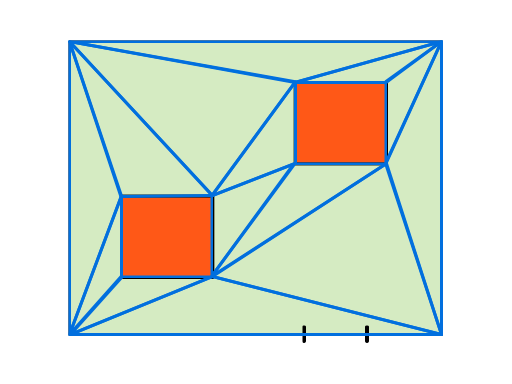
\includegraphics[width=\textwidth]{images/graph-generation/single/graph-generation-2}
 \caption{}
 \label{fig:graph-generation-b}
 \end{subfigure}
 ~
 \begin{subfigure}[b]{0.235\textwidth}
 
\includegraphics[width=\textwidth]{images/graph-generation/single/graph-generation-3}
 \caption{}
 \label{fig:graph-generation-c}
 \end{subfigure}
 ~
 \begin{subfigure}[b]{0.235\textwidth}
 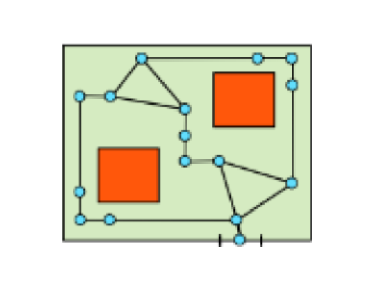
\includegraphics[width=\textwidth]{images/graph-generation/single/graph-generation-4}
 \caption{}
 \label{fig:graph-generation-d}
 \end{subfigure}
 
 \caption{Graph paths generation: 
 (a) detection of obstacles and computation of walkable area; 
 (b) triangulation of walkable area; 
 (c) identification of graph nodes area; 
 (d) junction of nodes.
 }
 \label{fig:graph-generation}
\end{figure*}

\subsection{HIJSON Class definition}\label{hijson-class-definition}

To exploit the possibilities offered by HIJSON Toolkit, along with the
HIJSON document, some custom dynamic behaviours must be described. These
behaviours encapsulate the specificities relative to comminucation
procols with the sensors as well as user interaction peculirities. The
interface for these behaviours is the HIJSON Class.

\begin{figure}[!h]
\centering
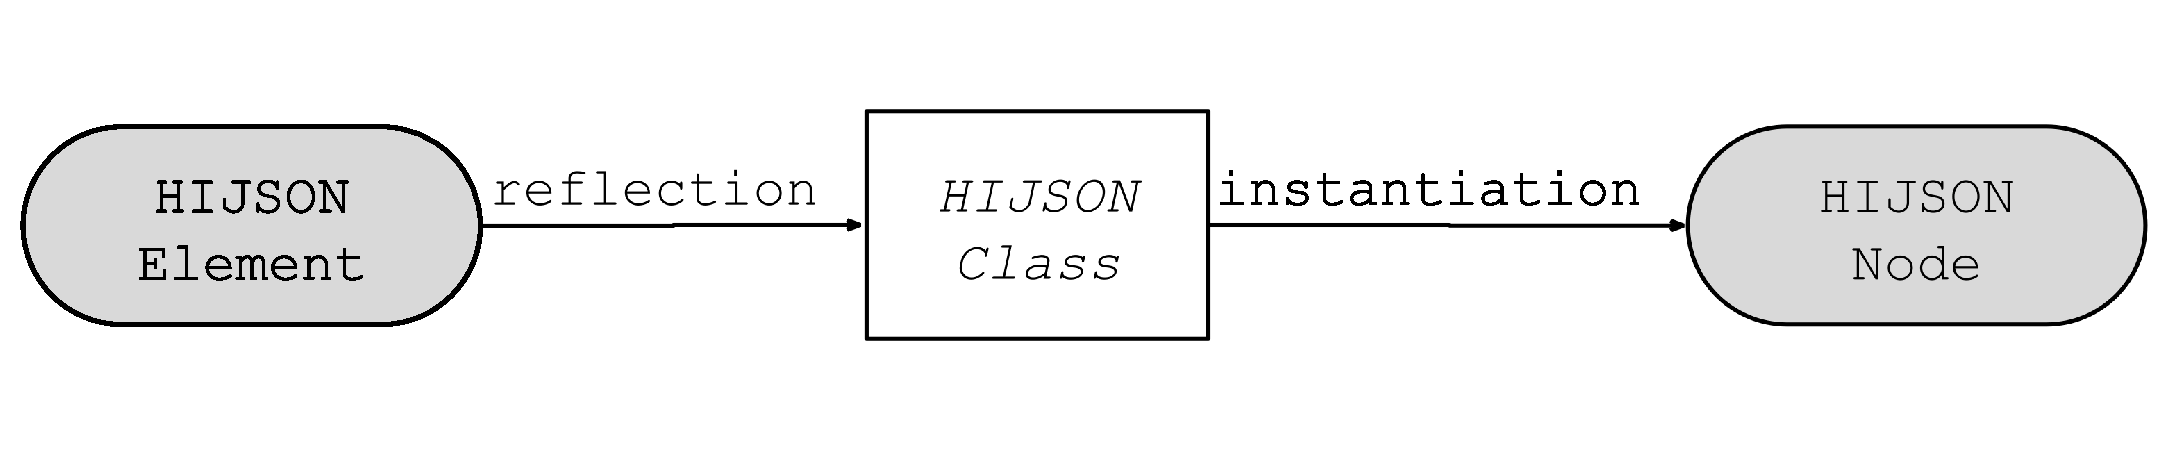
\epsfig{file=images/element-class-node.eps, width=0.44\textwidth}
\caption{HIJSON Element/Class/Node relashionship}
\label{fig:elem-class-node-rel}
\end{figure}

Each HIJSON Element of the HJSON document given as input, has a dynamic
counterpart, a running instance called HIJSON Node, instantiated
according to the corresponding HIJSON Class via relfection methods (see
figure \ref{fig:elem-class-node-rel}).

To specify a new HIJSON Class means to extend the Toolkit to deal with a
new class of HIJSON Element.

To extend the toolkit to deal with a new class of HIJSON Element is
required to to specify a new HIJSON Class, defining the following
properties and methods:

\begin{itemize}
\item
 \texttt{in\_graph}: a boolean value to express if the element is an
 approachable point in the graph paths;
\item
 \texttt{in\_2D\_map}: a boolean value to express if the element has 
 to be showd in the 2D map;
\item
 \texttt{get2DStyle}: a method that returns the 2D map appearence of
 the element, essentially HTML and CSS code;
\item
 \texttt{get3DModel}: a method that returns the 3D model appearence of
 the element, an instance of {\tt THREE.Object3D} of \emph{THREE.js} 
 framework;
\item
 \texttt{getWidget}: a method that returns the information widget, a
 \emph{React} component;
\item
 \texttt{getProxy}: a method that returns server side proxy which
 encapsulate IoT sensor communication protocol, a \emph{Node.js
 module}.
\end{itemize}

User's needs for new indoor elements, different sensor equipment,
alternative representation on 2D or 3D viewport are accepted by the
definition of new HIJSON Classes that allows in this way single point
custom extension of the Toolkit capabilities.


\begin{figure*}[htb]
\centering
% 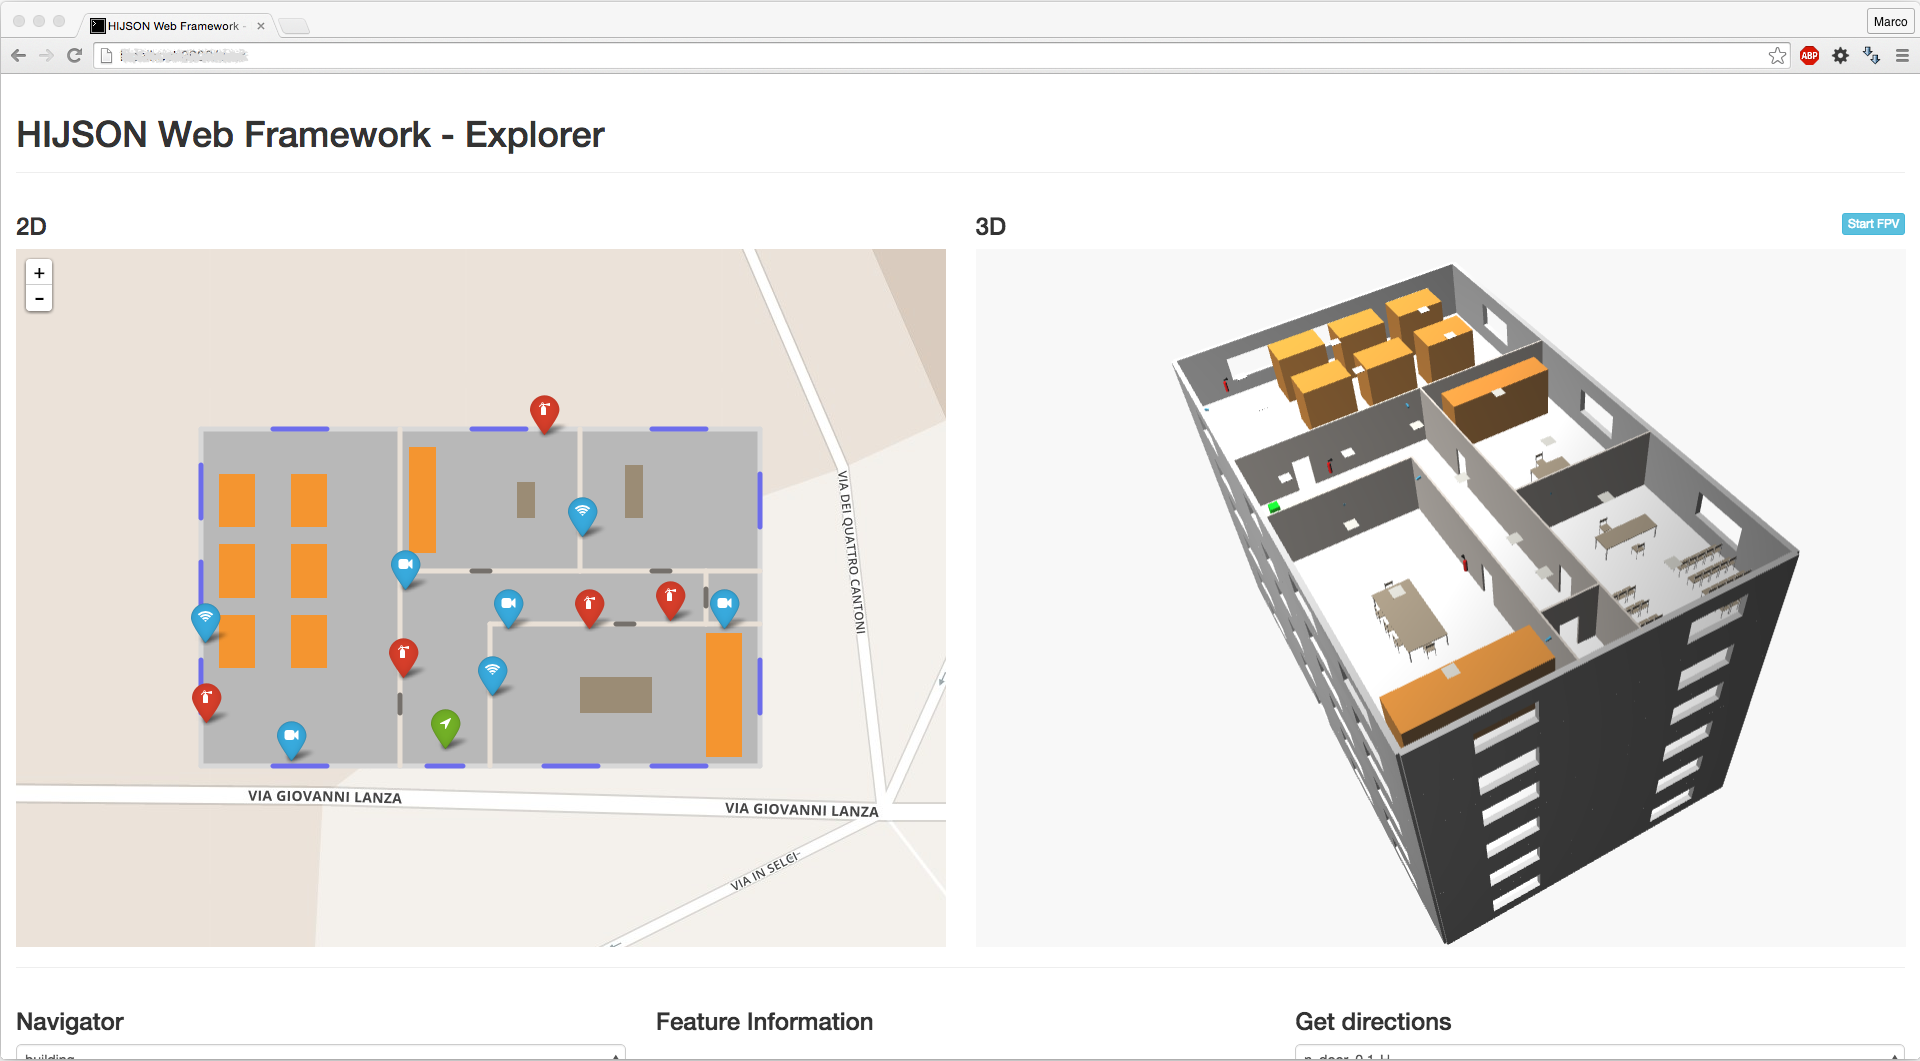
\includegraphics[width=\textwidth]{images/web_framework_1.png}
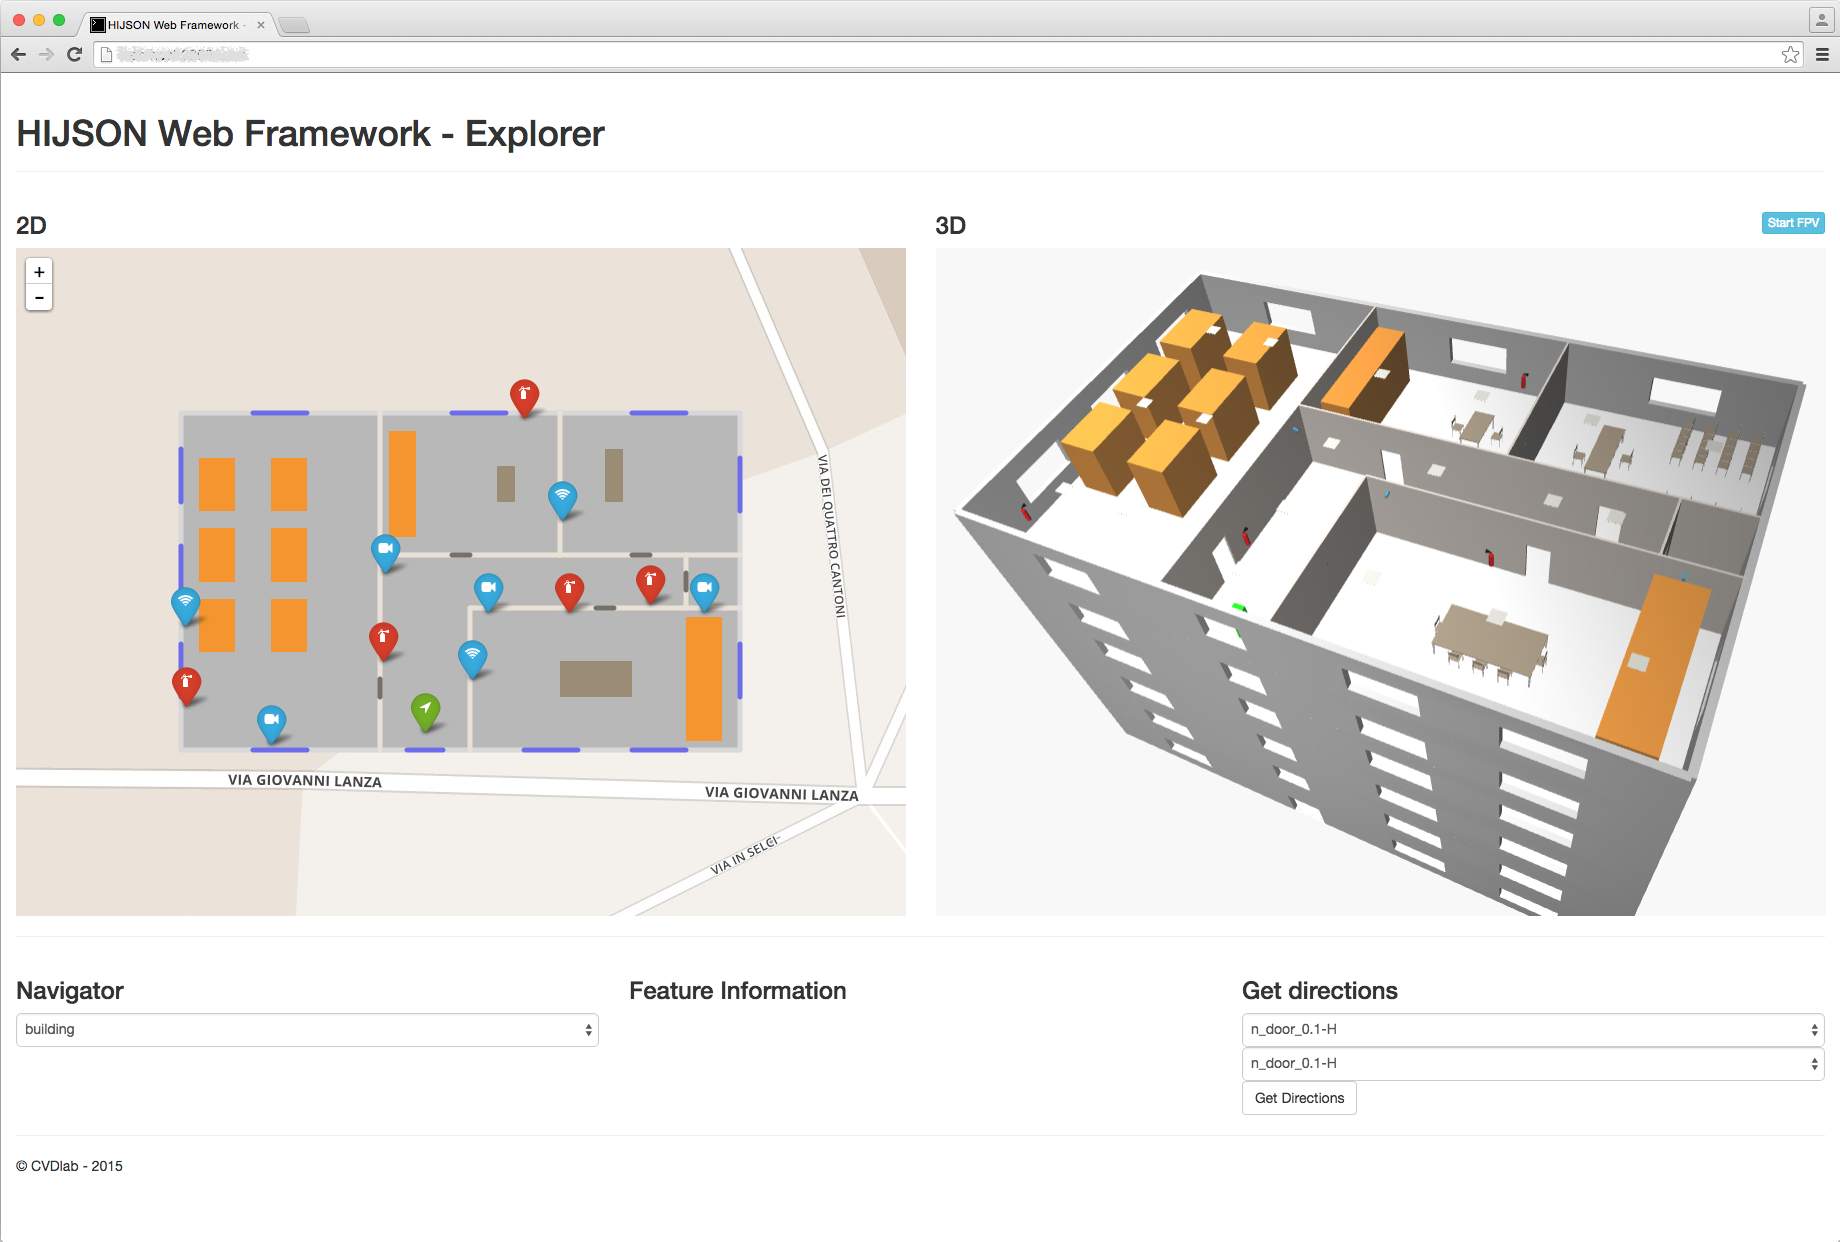
\includegraphics[width=\textwidth]{images/web_framework_2.png}
\caption{HIJSON Web Framework UI}
\label{fig:web-framework-ui}
\end{figure*}
